%****************************************************
%	CHAPTER 2 - Prototype Design
%****************************************************
\chapter{Prototype Design}
\label{ch:proto}
%====================================================
\section{Conventions Used}
\label{sec:proto.conventions}
The attitude conventions used for the system's dynamic derivations in the following Chapter:\ref{ch:dynamics} are first briefly discussed here. Often these aspects are omitted or assumed to be known already. It's important to clearly and unambiguously define a standard set of framing conventions to avoid uncertainty later. Rotation matrices are included but the focus remains on the \emph{contrast} between a rotation and transformation operation. Both \cite{spacecraftattitutdequaternions} and \cite{rigidbodylecture} provide an in depth and thorough explanation of rotation matrices and DCM attitude representation if such concepts are unfamiliar to the reader.
%====================================================
\subsection{Reference Frames Convention}
\label{subsec:proto.conventions.frames}
%====================================================
\begin{figure}[htbp]
\centering
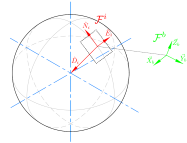
\includegraphics[width=0.6\textwidth]{figs/reference_frame}
\caption{Inertial and Body Reference Frames}
\label{fig:ref_frame}
\end{figure}
Euler (aerospace) frames are used for principle inertial and body coordinates (Fig:\ref{fig:ref_frame}). The inertial frame,~$\mathcal{F}^i$, is aligned such that the $\vec{X}_i$ axis is in the $\hat{N}$orth direction, $\vec{Y}_i$ is in the $\hat{E}$ast direction and $\vec{Z}_i$ is  in the $\hat{D}$ownward direction\footnote{In orbital sequences this would be toward the Earths' center. Sometimes referred to as the NED convention}. The body frame, $\mathcal{F}^b$, then has both $\vec{X}_b$ and $\vec{Y}_b$ aligned obliquely between two perpendicular arms of the quadrotor's body and the $\vec{Z}_b$ axis in the body's normal direction (Fig:\ref{fig:body-frame}). The body frame's axes and their relation to the prototype design are highlighted next in Section:\ref{subsec:proto.conventions.motoraxis}. Frame superscripts $i$ and $b$ represent inertial and body frames respectively whilst vector subscripts imply the reference frame in which the vector's coordinates exists in.
\par
Relative angular displacement between two frames is commonly measured by the three angle Euler set. The Euler angles $\Upsilon=[\phi ~\theta ~\psi]^T$ represents rotations about the $\vec{X}$,$\vec{Y}$ and $\vec{Z}$ axes respectively. Depending on how the rotation sequence is formulated, those angles can be used to construct rotation matrices which give relation to vectors or can transform coordinates. The generic equation to rotate a vector $\vec{v}$ about a (normalized) axis $\hat{n}$ by some angle $\mu$ is given by\footnote{Derived and proven in \emph{Quadrotor Dynamics and Control}\cite{quaddynamics}}:
\begin{equation}\label{eq:genrotationmatrix}
\vec{v}~'=\big(1-cos(\mu)\big)\big(\vec{v}\cdot \hat{n}\big)\hat{n}+cos(\mu)\vec{v}+sin(\mu)\big(\hat{n}\times\vec{v}\big)
\end{equation}
Which, when $\hat{n}$ is either $\vec{X}$,$\vec{Y}$ or $\vec{Z}$ axes, can be simplified to produce the fundamental rotation matrices $\mathbb{R}_x(\phi)$,$\mathbb{R}_y(\theta)$ and $\mathbb{R}_z(\psi)$. Multiplication by a rotation matrix $\mathbb{R}(\cdot)$ applies a left-handed \emph{rotation} operator, the resultant vector still exists in the same reference frame;
\begin{subequations} \label{eq:rotationoperator}
\begin{equation}\label{eq:rotationoperator.a}
\vec{v}~'=\mathbb{R}_{x}(\phi)\vec{v}
\end{equation}
\vspace{-20pt}
\begin{equation}\label{eq:rotationoperator.b}
\vec{v}~',\vec{v}\in\mathcal{F}^1
\end{equation}
\end{subequations}
\emph{\color{Gray} No subscripts are used in Eq: \ref{eq:rotationoperator} to indicate reference frame ownership because all vectors are in the same frame}
\par
A \emph{transformation} changes the vectors reference frame. The transformation is a rotation by an angle of the difference between the resulting and principle reference frames. A transformation from frame $\mathcal{F}^1$ to $\mathcal{F}^2$, differing by an angle of $\phi$ about the $\vec{X}$ axis is then:
\begin{subequations}\label{eq:transformationoperator}
\begin{equation}\label{eq:transformationoperator.a}
\vec{v}_2=\mathbb{R}_x(-\phi)\vec{v}_1
\end{equation}
\vspace{-20pt}
\begin{equation}\label{eq:transformationoperator.b}
\vec{v}_2\in\mathcal{F}^2~\text{and}~\vec{v}_1\in\mathcal{F}^1
\end{equation}
\end{subequations}
The distinction between Eq:\ref{eq:rotationoperator} and Eq:\ref{eq:transformationoperator} is the sense of the angular operand $\phi$, and hence the effect it has on the argument vector. The transformation of a vector from $\mathcal{F}^i$ to $\mathcal{F}^b$ is the product of three sequential operations about each axis. Because each subsequent rotation is applied relative to a new  intermediate frame, the sequence of axial rotation operations will effect the Euler set. Any consequences of that chosen order is something well documented in \emph{Quaternions and Rotation Sequence}, \cite{rotationsequences}. In this dissertation the Z-Y-X sequence is used. Hence a transformation of a vector $\vec{v}$ from the inertial to the body frame is applied by:
\begin{subequations}
\begin{equation}\label{eq:inertialbodytransformation.a}
\mathbb{R}_{i}^{b}\triangleq\mathbb{R}_z(\psi)\mathbb{R}_y(\theta)\mathbb{R}_x(\phi)
\end{equation}
\vspace{-15pt}
\begin{equation}\label{eq:inertialbodytransformation.b}
\vec{v}_b=\mathbb{R}_i^b(-\psi,-\theta,-\phi)\vec{v}_i
\end{equation}
\vspace{-15pt}
\begin{equation}\label{eq:inertialbodytransformation.c}
\Rightarrow\vec{v}_b=\mathbb{R}_z(-\psi)\mathbb{R}_y(-\theta)\mathbb{R}_x(-\phi)\vec{v}_i
\end{equation}
\vspace{-15pt}
\begin{equation} \label{eq:inertialbodytransformation.d}
\mathbb{R}_z(-\psi)\mathbb{R}_y(-\theta)\mathbb{R}_x(-\phi) \iff \mathbb{R}_x(\phi)\mathbb{R}_y(\theta)\mathbb{R}_z(\psi)=\mathbb{R}_{b}^{i}
\end{equation}
\end{subequations}
The relation in Eq:\ref{eq:inertialbodytransformation.d} is an inversion (\emph{transpose}) of the rotation matrix. A rotation matrix's inverse can be used interchangeably to maintain a positive sense of the rotational angle. To ensure clarity throughout this paper's mathematics, a negative angular sense implies a \emph{transformation} to a different reference frame. Where applicable, the order of rotation will indicate the sequence direction and an angular sign differentiates a rotation or transformation operation.
\par
An inherent singularity does exists with such attitude representations. Indeed Quaternions are used for kinematics later in lieu of Euler angles. Euler angular attitude representation is, however, easily understood and well suited to the conventional distinctions made here. Quaternion operations are similarly sequenced in the ZYX order:
\begin{subequations}
\begin{equation}
\mathbb{R}_i^b\iff Q_b^* \otimes (.) \otimes Q_b
\end{equation}
\vspace{-20pt}
\begin{equation}
Q_b^* \triangleq Q_z^* Q_y^* Q_x^*~\text{and}~Q_b \triangleq Q_x Q_y Q_z
\end{equation}
\end{subequations}
With $\otimes$ being the Hamilton product (or quaternion multiplier). Each quaternion, $Q_i$, is a unit quaternion about that $\hat{i}^{th}$ axis. The operator and subsequent quaternion kinematics are defined later in Sec: \ref{subsec:dynamics.rigidbody.quaternion}.
%====================================================
\subsection{Motor Axis Layout}
\label{subsec:proto.conventions.motoraxis}
%====================================================
Fundamentally the whole structure, although treated as rigid in the kinematics, consists of multiple bodies able to rotate relative to one another. Each propeller and motor pair is actuated by two servos. If the propeller, attached to the motors' rotor, has a rotational speed $\omega$ about the $\vec{Z}$ stator axis, then two servos are aligned with $\vec{Y}$ and $\vec{X}$ axes to pitch and roll the propeller away from its principle rotational axis. Each of the four motors has their own reference frame, $\mathcal{F}^{M_i}$, aligned as in Fig:\ref{fig:motor-axes}.
\begin{figure}[htbp]
\centering
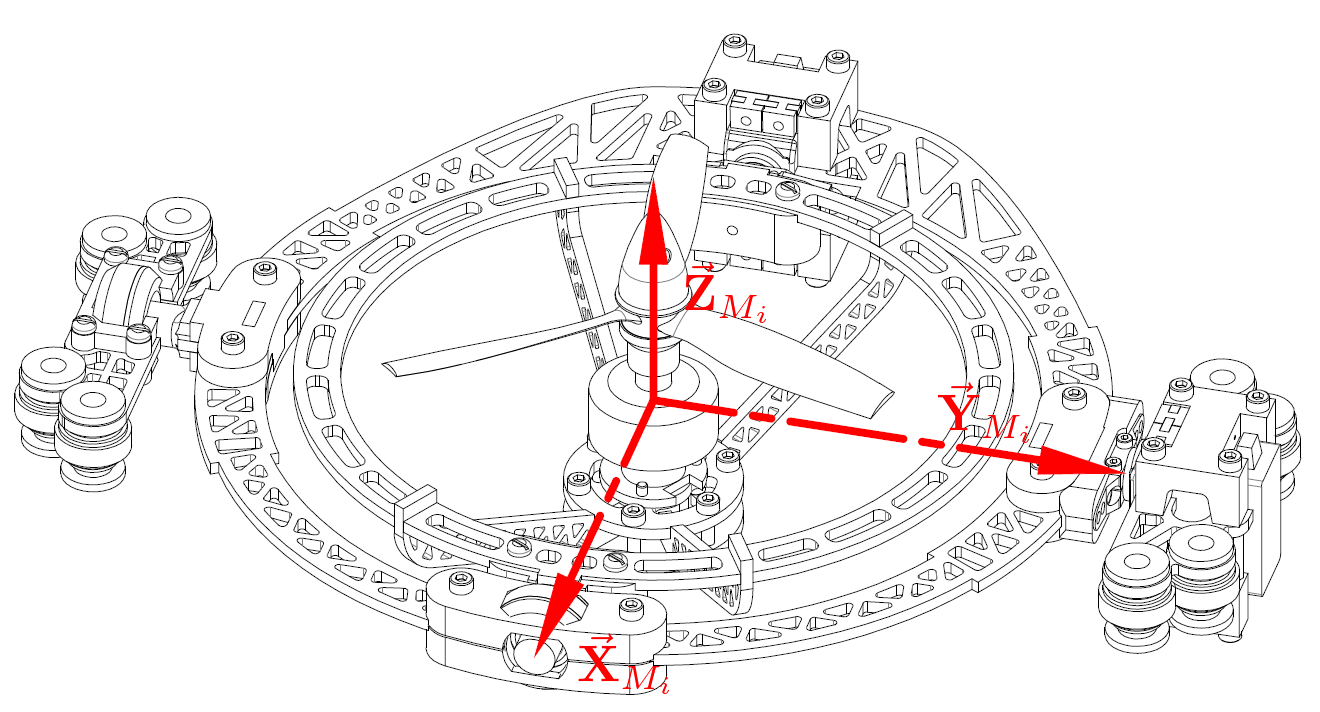
\includegraphics[width=0.8\textwidth]{figs/motor-axes}
\caption{Aligned Motor Frame Axes}
\label{fig:motor-axes}
\end{figure}
\par
The motor frames, numbered $1-4$, transform to the body frame first by an angle of $\lambda_i$ about the $\vec{X}_{M_i}$ axis. Then by $\eta_i$ about the $\vec{Y}_{M_i'}$ axis in an intermediate $M_i'$ frame. The second servo actuates $\eta_i$ to produce a second intermediate frame $M_i''$, the servo is fixed in the $M_i'$ frame. Finally there is a relative $\vec{Z}_{M_i''}$ rotation between $\mathcal{F}^b$ and $\mathcal{F}^{M_i''}$. The layout of all four motor modules are such that the $\vec{Z}$ axis transformation between the intermediate frame $\mathcal{F}^{M_i''}$ and $\mathcal{F}^b$ are all constants; $0,~90^{\circ},~180^{\circ}~\text{or}~270^{\circ}$. Each modules' state is fully described by $[\Omega_{i},~\lambda_{i},~\eta_{i}]^{T}$ for $i\in [1:4]$.
\begin{figure}[hbtp]
\centering
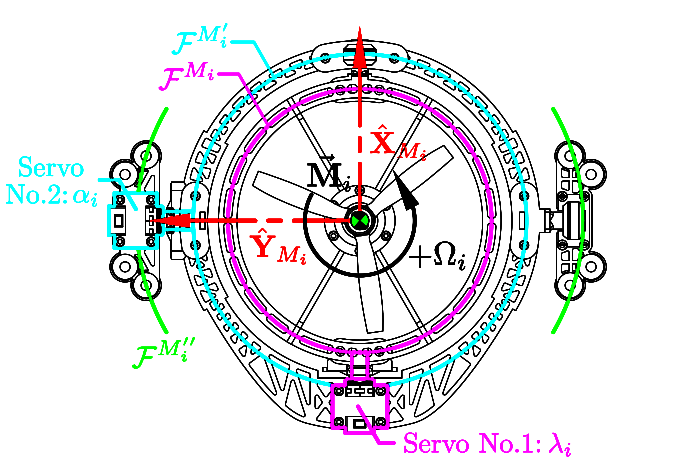
\includegraphics[width=0.6\textwidth]{figs/motor-frame}
\caption{Intermediate Motor Frames}
\label{fig:motor-frame}
\end{figure}
\par
The four motor modules are aligned relative to the body's XYZ axes as show in Fig:\ref{fig:body-frame}. Modules 1 and 3 have their X-axes respectively in the positive and negative X direction of the body frame. Similarly Modules 2 and 4 have their X-axes in the positive and negative Y directions of the body frame.
\begin{figure}[htbp]
\centering
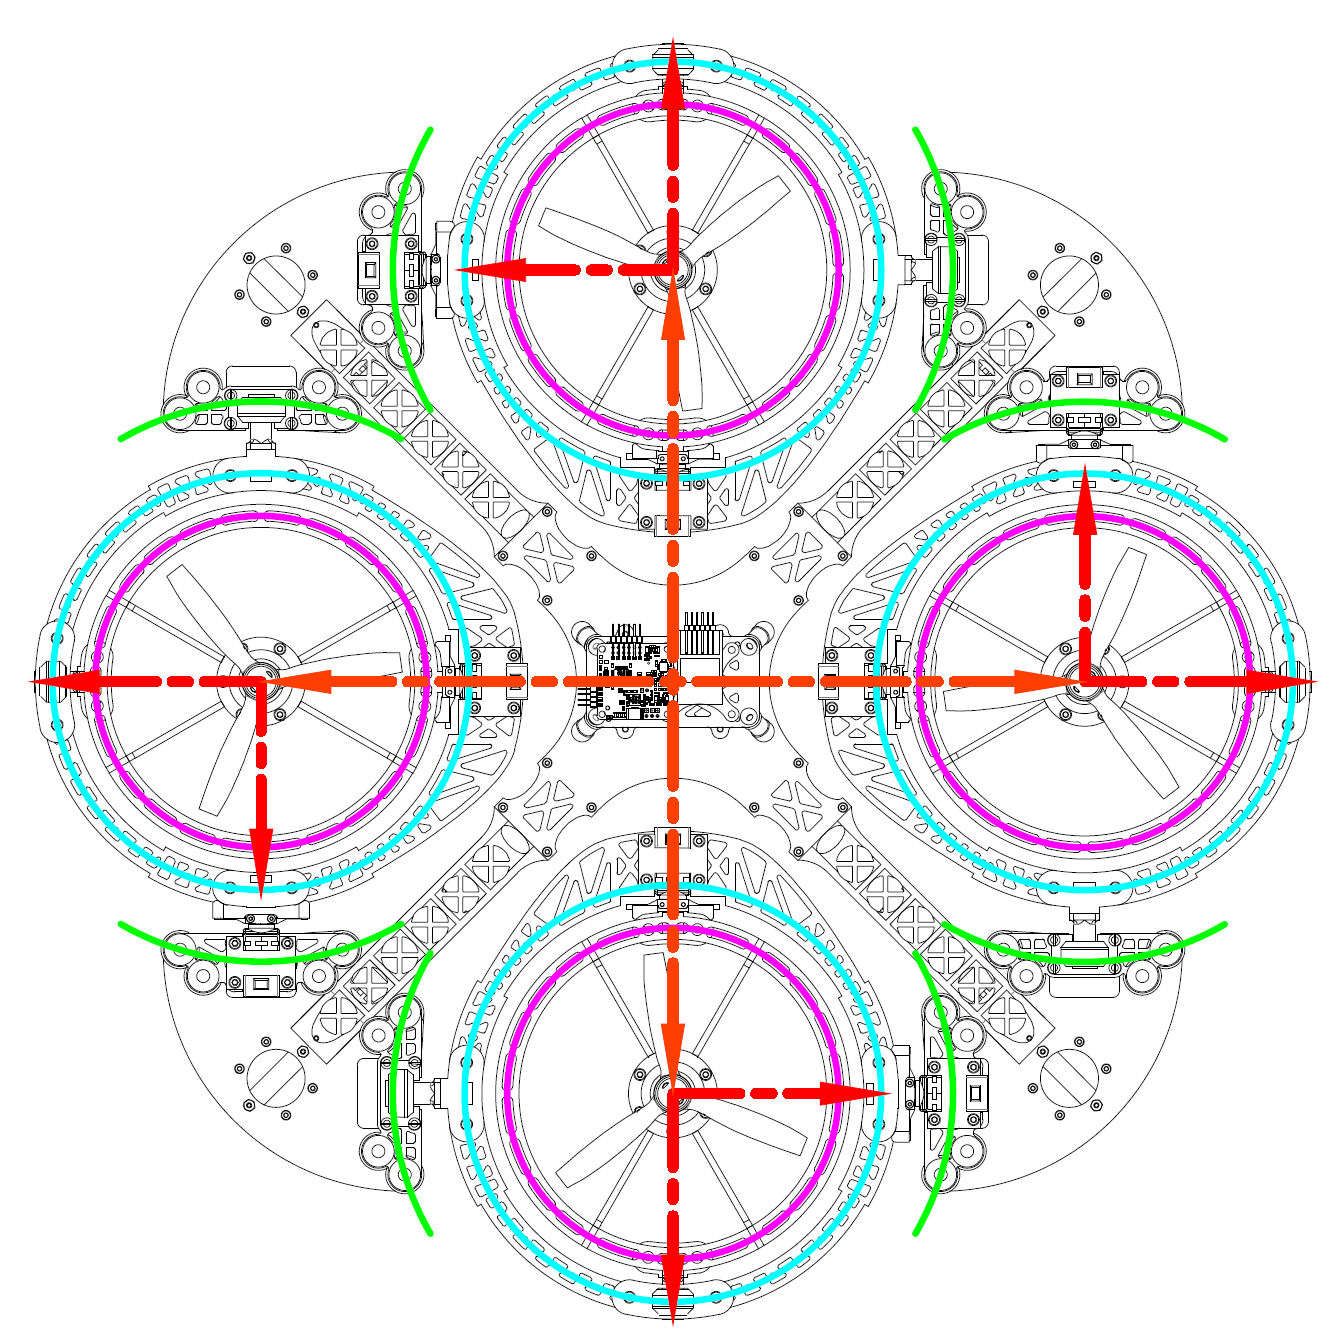
\includegraphics[width=0.75\textwidth]{figs/body-frame}
\caption{Body Frame Axes Layout}
\label{fig:body-frame}
\end{figure}
\par
\emph{\color{Gray}Not shown in Fig:\ref{fig:body-frame} is the relative Z axis position with respect to the structure. The Z height of the body's motion centroid such that its origin is co-planar with the four motor modules rotational centres. The centre of motion is not the center of mass, an aspect which is quantified in the following Section:\ref{subsec:proto.design.inertia}.}\\ Transformation relationships from each of the motor frames to the body can be characterized as:
\begin{subequations}
\begin{equation}\label{eq:motor-module-rotation.a}
\vec{v}_b=\mathbb{R}_z(-\sigma_i)\mathbb{R}_y(-\eta_i)\mathbb{R}_z(-\lambda_i)\vec{v}_{M_i},~\sigma_i\in[0, 90^{\circ}, 180^{\circ}, 270^{\circ}]
\end{equation}
\vspace{-15pt}
\begin{equation}\label{eq:motor-module-rotation.b}
\mathbb{R}_z=\begin{bmatrix}
1 & 0 & 0\\
0 & 1 & 0\\
0 & 0 & 1
\end{bmatrix}, \begin{bmatrix}
0 & -1 & 0\\
1 & 0 & 0\\
0 & 0 & 1
\end{bmatrix}, \begin{bmatrix}
-1 & 0 & 0\\
0 & -1 & 0\\
0 & 0 & 1
\end{bmatrix}, \begin{bmatrix}
0 & 1 & 0\\
-1 & 0 & 0\\
0 & 0 & 1
\end{bmatrix}~\text{for}~i\in[1,2,3,4]~\text{respectively}
\end{equation}
\label{eq:motor-module-rotation}
\end{subequations}
The entire actuator space, including propeller speed $\Omega_i~[rps]$, is then ($\in\mathbb{R}^{12}$)\footnote{Disambiguation: An omission of axial subscript on the $\mathbb{R}$ symbol implies a real space of the superscript dimension.}, or rather $\mathbb{U}\in\mathbb{R}^{12}$. The actuator input set $u \in \mathbb{U}$ is then structured as:
\begin{equation}
u_{\in\mathbb{U}}=\big[ \Omega_{1} ~ \lambda_{1} ~ \eta_{1} ~ \ldots ~ \Omega_{4} ~ \lambda_{4} ~ \eta_{4}  \big]^T
\end{equation}
\newpage
%====================================================
\section{Design}
\label{sec:proto.design}
%====================================================
\begin{figure}[htbp]
\centering
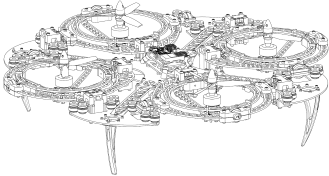
\includegraphics[width=\textwidth]{figs/iso-design}
\label{fig:iso-design}
\caption{Isometric layout of the designed prototype}
\end{figure}
The actual prototype went through a series of different design iterations, all aimed at using as many off-the-shelf RC components as possible whilst attempting to optimize construction costs. A significant factor in the design was the net weight whose upper limit, as mentioned before, is inherently linked to the thrust produced by the motors used. Some of the more important design aspects, like inertias, are discussed here in order to give context to some of the dynamics derived in the next chapter. The actuator suite's functionality and transfer characteristics are presented here. Finally a brief overview of the electrical systems layout is given with the components associated electrical characteristics listed. A review of the physical prototype realized and control loop implementation is detailed in Chapter:\ref{ch:flight}~along with actual flight test results.
%====================================================
\subsection{Actuation}
\label{subsec:proto.design.actuation}
%====================================================
\begin{figure}[hbtp]
\begin{subfigure}{.5\textwidth}
\centering
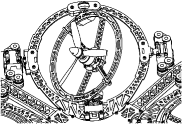
\includegraphics[width=\textwidth]{figs/motor-assembly}
\caption{Motor Module Assembly}
\label{fig:motor_assembly}
\end{subfigure}
\begin{subfigure}{.5\textwidth}
\centering
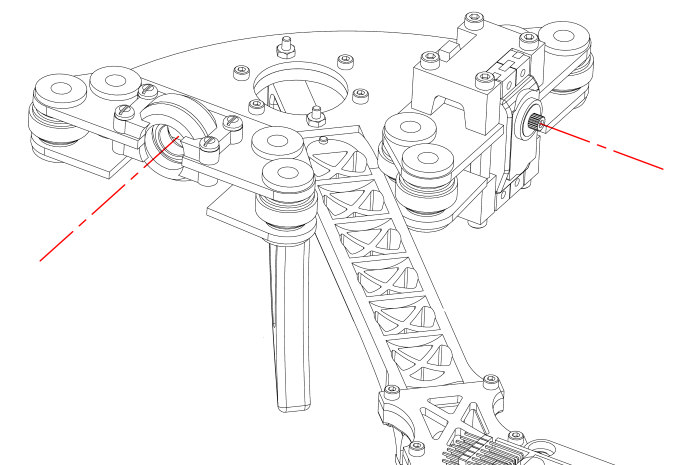
\includegraphics[width=\textwidth]{figs/motor-support}
\caption{Motor Frame Damping Support Assemblies}
\label{fig:motor_support}
\end{subfigure}
\caption{Motor Assembly}
\end{figure}
The novel component of the design is articulation of each motor module, independently redirecting the thrust generated by each lift propeller. Within each module are servos affixed onto sequential rings to pitch and roll the substructure's axes. The gyroscope-like frame that surrounds each motor/propeller pair accommodates the relative movement. Aligned with each servo is a coaxial support bearing. The coaxial bearing and actuator servos do have a mass disparity that results in an eccentric mass center, producing a gravitational torque arm. Unfortunately, due to weight constraints, counter balance measures cannot be introduced. Consequences from the center of mass variations must either be compensated for (\emph{plant dependent solution}) or exploited in the dynamics (\emph{additional non-linear actuator plants}). The precise effects are quantified numerically next in Section:\ref{subsec:proto.design.inertia}.
\par
Each module is designed such that thrust vector produced coincides with the two rotational axes intersections (Fig:\ref{fig:motor_assembly}). There's no perpendicular displacement of generated thrust vectors relative to the body's X-Y-Z origin\footnote{Although the center of gravity does have a time varying position dependent on the 8 servos positions}. It's more prudential to ensure intersection of the thrust vector with the rotational center than to balance the masses undergoing rotation. A thrust varying torque is harder to compensate for than a gravitational torque given the complexity with modelling a propeller's aerodynamic thrust (Section:\ref{subsec:dynamics.aero.bem}).
\par
The primary frame has silicon damping balls between brackets which attach to the motor gyroscope assembly (Fig:\ref{fig:motor_support}). For damping to be effective there has to be roughly equatable relative masses between the two damped bodies. A smaller damping assembly in the center of the frame houses all the electronics and power distribution circuitry. All the mounting brackets which affix the motor moduels are 3D printed from CAD models using an Ultimaker V2+\cite{ultimaker}. There is a complete bill of materials for all parts used, including working drawings for each 3D printed bracket and the laser cut frame(s), in Appendix:\ref{app:bom}.
\par
\begin{figure}[hbtp]
\centering
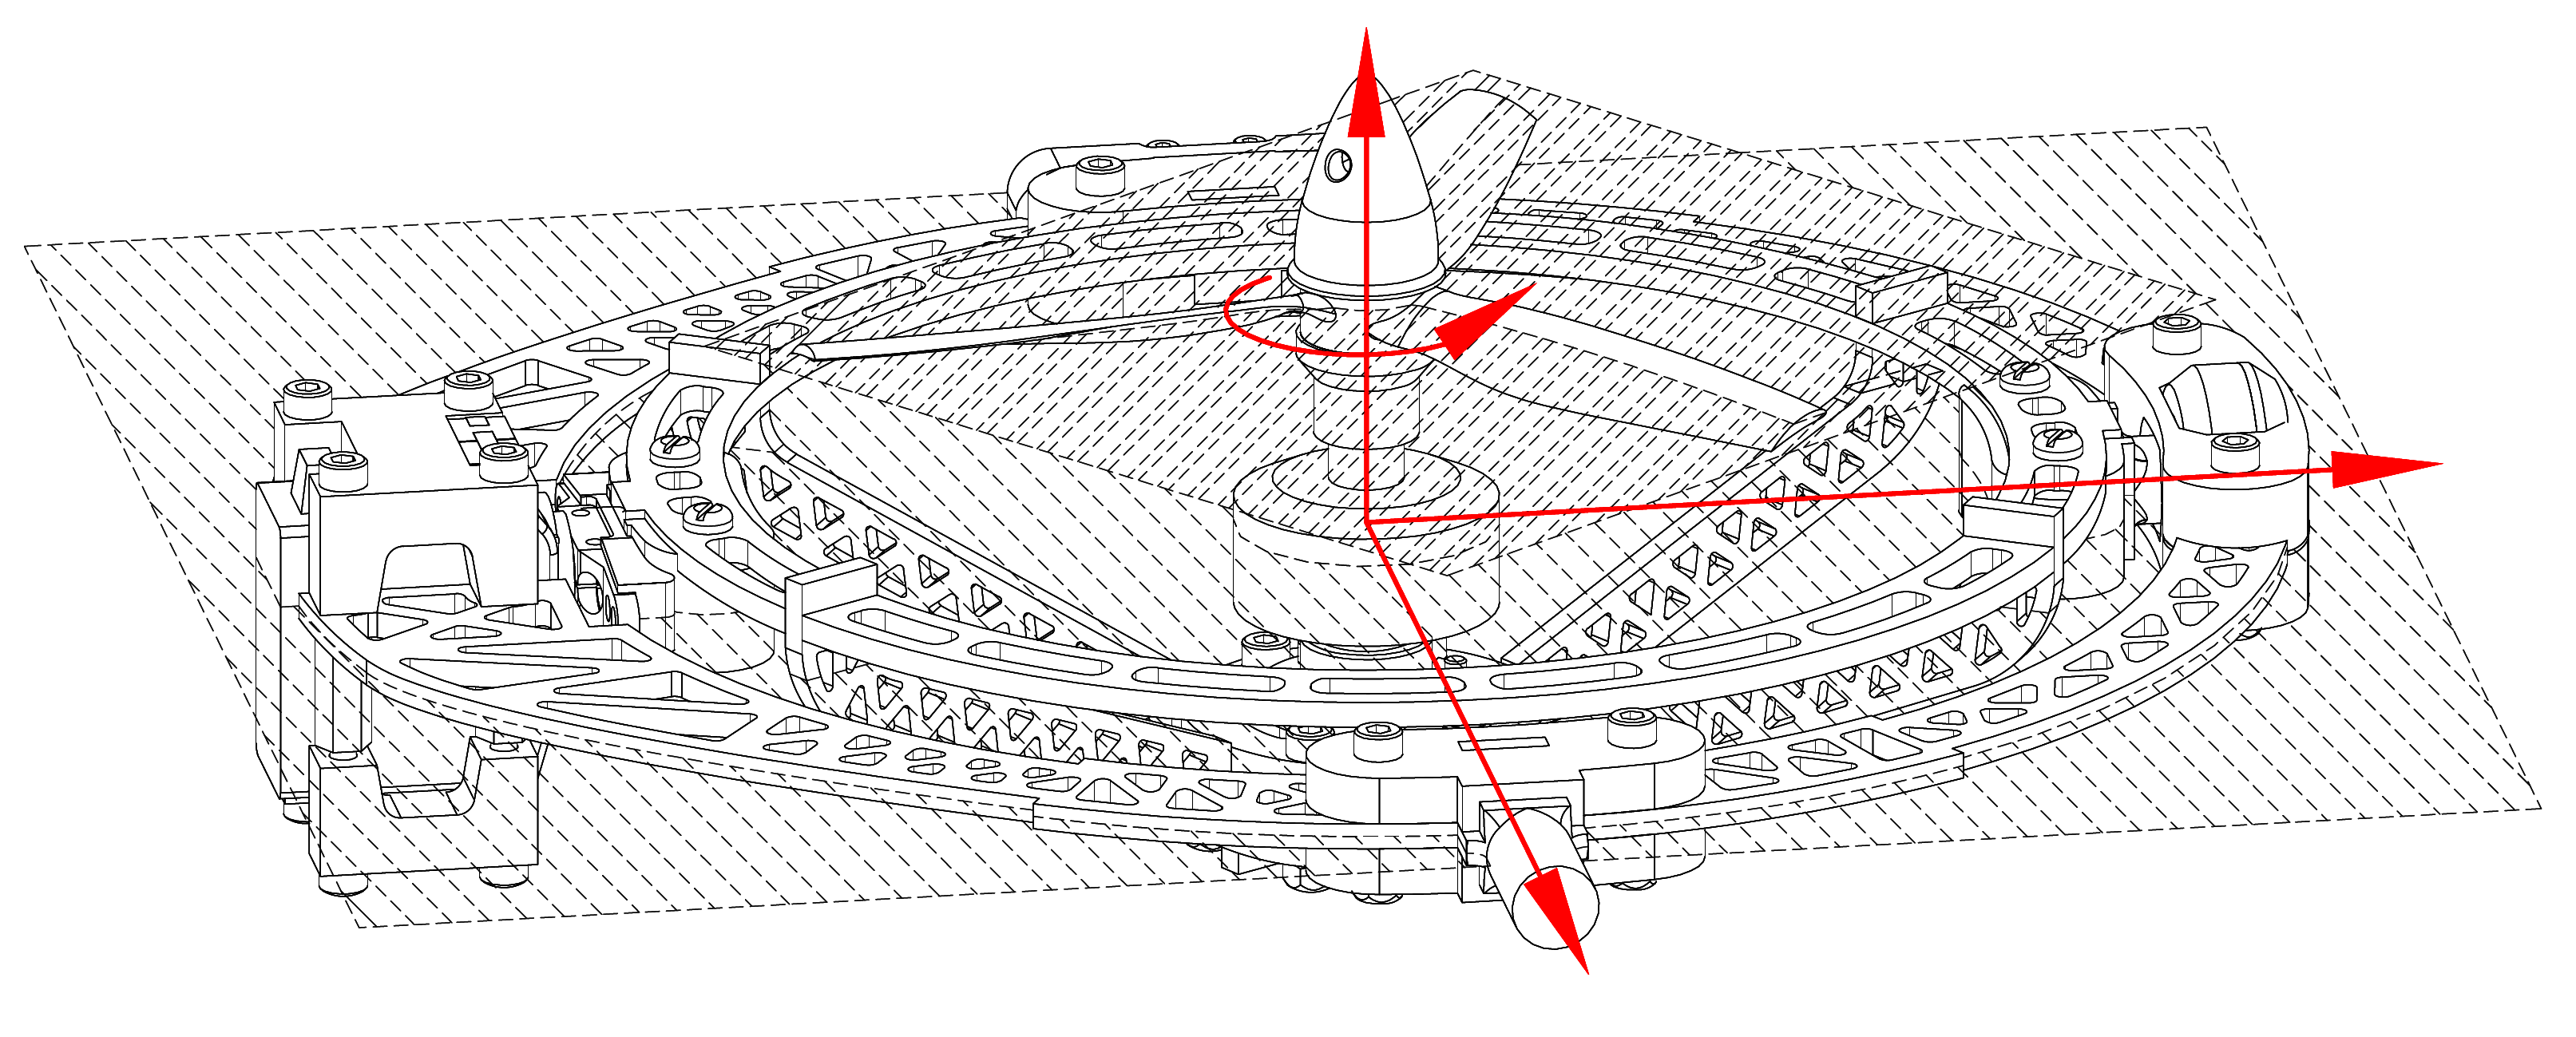
\includegraphics[width=\textwidth]{figs/motor-prop}
\caption{Difference between propeller and motor planes}
\label{fig:motor_prop}
\end{figure}
The propellers rotational plane is not exactly the aligned with the plane made by the $\vec{X}_{M_i}$ and $\vec{Y}_{M_i}$ rotational servo axes (Fig:\ref{fig:motor_prop}). The offset is approximately 28.2 mm and must be considered when evaluating pitch/roll gyroscopic torque responses later in Section:\ref{subsec:dynamics.nonlinearities.gyrotorques}. The propellers are 6 inch ($6 \times 4$) 3-Blade plastic Gemfam propellers, powered Turnigy DST-700KV Outrunner Brushless DC motors. The thrust produced as a funciton of angular velocity (in RPS) for the propellers is derived in Section:\ref{subsec:dynamics.aero.bem}. The BLDC motors are controlled with Hobbywing XRotor 15A ESC modules with an inline Orange RPM Sensor. The transfer function for the combined unit is presented subsequently in Section:\ref{subsec:proto.design.transfer}. Power for the quadrotor is supplied not from a battery bank but from a power tether. Tethered power will ensure consistent flight time and reduce the concern of payload strain on the available lift actuation. Power lines to both the BLDC motors and servos are both supplied conventionally, however an ideal construction would see slip-rings for each module's supply. Power transmission lines are affixed such that they don't impede rotation. 
\begin{figure}[htbp]
\centering
\begin{subfigure}{0.49\textwidth}
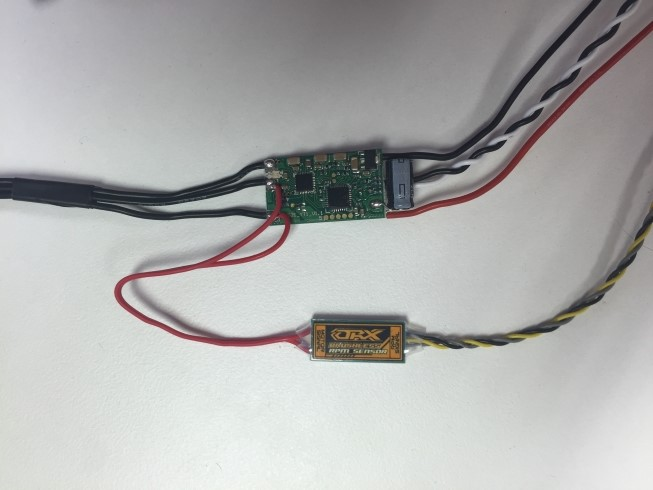
\includegraphics[width=\textwidth]{figs/motor-esc}
\caption{BLDC ESC \& RPM Sensor Assembly}
\label{fig:bldc-esc}
\end{subfigure}
\begin{subfigure}{0.49\textwidth}
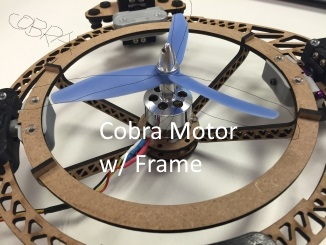
\includegraphics[width=\textwidth]{figs/motor-bldc}
\caption{Turnigy DST-700KV BLDC Motor}
\label{fig:bldc-motor}
\end{subfigure}
\end{figure}
\par
Metal gear Corona DS-339MG digital servos are used for the two axes of rotation (Fig:\ref{fig:motor-servo}). Each servo has a range of $180^{\circ}$, positioned such that a $\text{zero}^{\text{th}}$ offset aligns the motor modules  adjacent to the body frame and has a $\pm 90^{\circ}$ range. A digital servo updates at 330 Hz, faster than a 50 Hz analogue servo equivalent (Table:\ref{tab:servo}). This means the otherwise $20$ms zero-order analogue sampling becomes a less significant $3.30$ms zero-order holding time. Both the $\vec{X}_{M_i}$ and $\vec{Y}_{M_i}$ axis servos will be rotating a large loading mass and so their \emph{open loop} plant dynamics are determined empirically in Section:\ref{subsec:proto.design.transfer} using test data included in Appendix:\ref{app:systemdat}.
\begin{table}[h]
\centering
\fbox{
\begin{minipage}{0.7\textwidth}
\begin{tikztimingtable}
50 Hz: &[C] 31{C} G\\
Analogue Servo &1{L} 1.5{H} 18.5{L} 1.5{H} 10{L}\\
Digital Servo&1{L} 15{1.5{H} 1.53{L}}\\
\end{tikztimingtable}
\end{minipage}
}
\caption{Analogue \& Digital Timing Signals}
\label{tab:servo}
\end{table}
\begin{figure}[htbp]
\centering
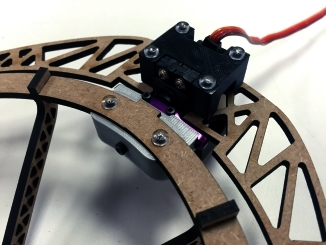
\includegraphics[width=0.5\textwidth]{figs/motor-servo}
\caption{Corona Servo Bracket}
\label{fig:motor-servo}
\end{figure}
%====================================================
\subsection{Inertial Matrices \& Mass}
\label{subsec:proto.design.inertia}
%====================================================
\emph{\color{Gray} Although inertias are presented here rounded to either 2 or 0 decimal places, full floating point numbers are used in simulation and prototype software. Un-rounded inertias are included in Appendix:\ref{app:eq}. Similarly rotation matrices produce a more cumbersome results for Eq:\ref{eq:inertia.middle}\ref{eq:module-inertia}\ref{eq:body-inerta}, which are susceptible to singularities. Quaternion operators are used in practice.}
\subsubsection*{Inertias}
An undesirable side effect of the rigid body rotations the structure undergoes are the inertial responses produced from such movements. Given Newton's Second Law of rotational motion$^{\dagger}$, the applied rotations are going to produce an equal but opposite reaction onto the principle inducing frame. Similarly a gyroscopic cross product from rotational velocities is also present. Such first and second order effects are often neglected given that angular rates are mostly small enough to approximate as zero, $\vec{\omega}_b\approx\vec{0}$. A dynamic set-point (non-zero) attitude tracking plant is, however, going to produce sizable time varying body angular velocities and accelerations. Unlike a traditionally actuated quadrotor, such effects have to be accounted for.
\begin{figure}[htbp]
\centering
\begin{subfigure}{0.49\textwidth}
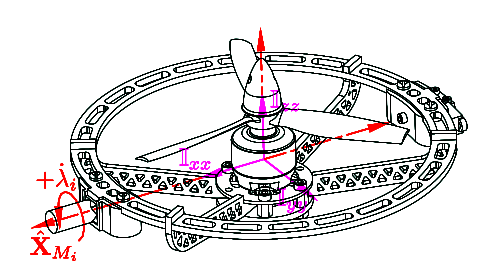
\includegraphics[width=\textwidth]{figs/inertia-inner}
\caption{Inner Ring Rotational Structure}
\label{fig:inertia-inner}
\end{subfigure}
\begin{subfigure}{0.49\textwidth}
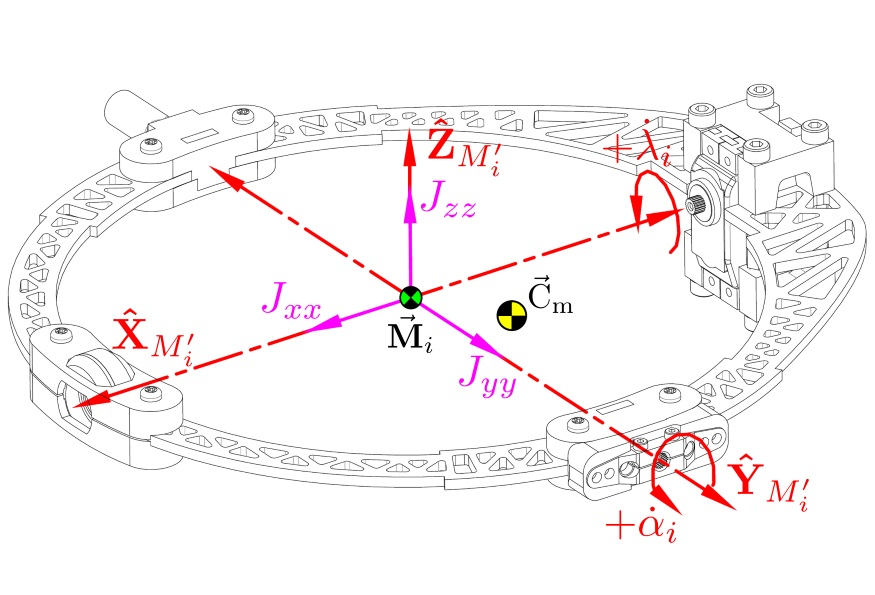
\includegraphics[width=\textwidth]{figs/inertia-middle}
\caption{Middle Ring Rotational Structure}
\label{fig:inertia-middle}
\end{subfigure}
\caption{Inertial Measurement References}
\end{figure}
\par
The manifestation of the aforementioned torques are explored in thorough detail in Section:\ref{sec:dynamics.nonlinearities}. Those effects are both dependent on the rotational body's inertial tensor\footnote{All inertias are assumed asymmetrical and calculated in Solidworks with overridden masses to match physical prototype measurements in App:\ref{app:bom}} about the respective rotational axes. The magnitude of those inertias are obviously a byproduct of the structure's design. Starting with the innermost assembly, in each Motor Frame $\mathcal{F}^{M_i}$, the inside ring structure is a 99g assembly (all components incorporated). The rotational center \emph{roughly} coincides with the center its of mass ($C.M=\begin{bmatrix}
-1.40 &  -0.04 & -1.94\\
\end{bmatrix}^T~~[mm]$ relative to its rotational center). The inner ring being rotated by $\lambda_i^{~\circ}$ about the $\vec{X}_{M_i}$ axis then has an inertial matrix (centered as in Fig:\ref{fig:inertia-inner}):
\begin{subequations}\label{eq:inertia.inner}
\begin{equation} \label{eq:inertia.inner.a}
\mathbb{I}_{M_i}=\begin{bmatrix}
588.84 & -0.28 & 0.25\\
-0.28 & 1966.60 & 0.90\\
0.25 & 0.90 & 2141.78\\
\end{bmatrix}~~[g.cm^2]
\end{equation}
\vspace{-5pt}
\begin{equation} \label{eq:inertia.inner.b}
\approx diag\big(588, ~1966, ~2141\big)\times10^{-7}~~[kg.m^2]
\end{equation}
\end{subequations}
The effect of a rotating propeller on the inertia in Eq:\ref{eq:inertia.inner.a} is approximated by a solid disc and hence the inner ring's inertial products are regarded as negligible. The moment of inertia about that $\vec{X}_{M_i}$ axis, pertinent to $\lambda_i$ rotation, is then $\mathbb{I}_{\lambda}=588.84\times10^{-7}~~[kg.m^2]$.
\par
The first $\lambda_i$ actuating servo and bearing supports are affixed to the intermediate middle ring assembly (Fig:\ref{fig:inertia-middle}). The middle ring frame, $\mathcal{F}^{M_i'}$, is a 102g structure, excluding the inner most ring. Collectively the mass for both the inner and middle rings structures is $m_{module}=201g$. That middle ring is rotated by $\eta_i^{~\circ}$ about its $\vec{Y}_{M_i}$ axis. The compound body's inertia about the axis of rotation, $\vec{Y}_{M_i}$, is a combination of both the middle ring's inertia and the inner ring's.  The latter contribution being a function of the \emph{rotation} (not transformation) angle $\lambda_i^{~\circ}$ which, from the conservation of angular momentum theory \cite{rigidbodyinertia}\footnote{$\mathbb{R}_x$ is a full rank and square, so an inverse $\mathbb{R}^{-1}_{X}$ always exists}, is:
\begin{subequations}\label{eq:inertia.middle}
\begin{equation} \label{eq:inertia.middle.a}
\text{If} ~~\mathbb{I}_{middle}=\begin{bmatrix}
3024.30 & 0.03 & 406.84\\
0.03 & 8791.16 & 0.01\\
406.87 & 0.01 & 11579.85\\
\end{bmatrix}~~[g.cm^2]
\end{equation}
\vspace{-5pt}
%Off diagonal elements, inertia products, have a different formula?
\begin{equation}\label{eq:inertia.middle.b}
\mathbb{I}_{M_i'}=\mathbb{I}_{middle}+\mathbb{R}_{X}(\lambda_i)\big(\mathbb{I}_{inner}\big)\mathbb{R}_{X}^{-1}(\lambda_i)
\end{equation}
\vspace{-10pt}
\begin{equation}\label{eq:inertia.middle.c}
\mathbb{I}_{M_i'}(\lambda)=\mathbb{I}_{const}+\mathbb{I}_{M_i}(\lambda)
\end{equation}
\vspace{-10pt}
\begin{equation} \label{eq:inertia.middle.d}
\approx\begin{bmatrix}
3609 & 0 & 407\\
0 & 10842 & 0\\
407 & 0 & 13630\\
\end{bmatrix}
+
\begin{bmatrix}
0 & 0 & 0\\
0 & -88{c}_{2\lambda} & 2{c^2}_{\lambda}-91s_{2\lambda}\\
0 & 2{c^2}_{\lambda}-91s_{2\lambda} & 88{c}_{2\lambda}\\
\end{bmatrix}
\times10^{-7}~~[kg.m^2]
\end{equation}
\end{subequations}
With $\mathbb{I}_{inner}=\mathbb{I}_{M_i}$ being the inertia from Eq:\ref{eq:inertia.inner.a}, transformed by a rotation $\mathbb{R}_x(\lambda_i)$. The net inertia being a function of rotation angle, $\lambda_i$, and a constant inertia (Eq:\ref{eq:inertia.middle.c}) is then simplified\footnote{Eq:\ref{eq:inertia.middle.d} is rounded to no decimal places, seeing that its units are already $\times10^{-7}$} to Eq:\ref{eq:inertia.middle.d}. It's important to note the non-zero product of inertia, $\mathbb{I}_{yz}$, which is going to result in a $\tau_z$ response. The inertia then encountered by an $\eta_i$ rotation is:
\begin{equation}\label{eq:inertia.middle.vpa}
\mathbb{I}_\eta(\lambda)\approx[0,~ 10842-88{c}_{2\lambda},~ 2{c^2}_{\lambda}-91s_{2\lambda}]^T\times10^{-7}~~[kg.m^2]
\end{equation}
\par
Variable inertias dependent on state input variables are the first of many non-trivial aspects unique to this aircraft's design. The resultant control solutions are thus decidedly plant dependent in their formulation. Secondly, the center of mass for the motor module's compound assembly isn't coincidental with either rotational axes intersection. As a result the effective center of mass for the entire structure is going to be time varying, dependent on the angular rotation which the motor modules have been effected by.
\par
\begin{figure}[htbp]
\centering
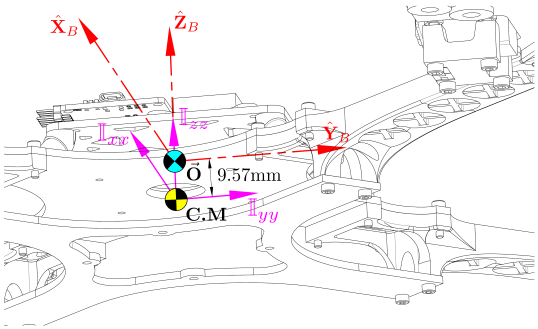
\includegraphics[width=0.7\textwidth]{figs/inertia-center}
\caption{Body Frame Center of Mass}
\label{fig:inertia-center}
\end{figure}
The second $\eta_i$ rotating servo joins the complete motor module (both the inner and middle ring assemblies) to the body structure. The inertial volume of the servo and bearing supports contribute then to the body's inertia, whose value excludes any of the four motor modules. Consisting of servo and bearing damping brackets, the "damping" assembly collectively weighs 84g and suspends the motor modules from the body frame with a set of silicon damping balls. The body assembly's center of mass (Fig:\ref{fig:inertia-center}) coincides with the XY directional axes and lies $\Delta Z=-14.27~mm$ below the Body Frame's origin of motion, $\vec{O}\in\mathcal{F}^b$.
\\
\emph{\color{Gray}Note: the origin which all motion is calculated with respect to is co-planar to the motor module's rotational centers, \underline{not} the net center of mass.}
\newpage
The body's weight, including all four damping assemblies, totals to $814.7 g$. The body's net inertia (\emph{sans} motor modules) $\mathbb{I}_{body}$, about its center of mass is:
\begin{subequations}\label{eq:inertia.body}
\begin{equation}\label{eq:inertia.body.a}
\mathbb{I}_{body}=\begin{bmatrix}
182018.63 & -0.44 & -80.30\\
-0.44 & 181896.17 &	-17.75\\
-80.30 & -17.75 & 360077.58\\
\end{bmatrix}~~[g.cm^2]~\text{or}~\times10^{-7}~[kg.m^2]
\end{equation}
Using the Parallel Axis theorem$^{\dagger}$, that same net body inertia about the body frame's origin, $\vec{O}_b$, is:
\begin{equation}\label{eq:inertia.body.b}
{\mathbb{I}_{body}}'=\mathbb{I}_{body}+m(\vec{d}\cdot\vec{d}+\vec{d}\otimes\vec{d}^T)\approx\mathbb{I}_{body}+md^2
\end{equation}
Here $\otimes$ represents the Hamilton product of two 3X3 matrices, used later in Chapter:\ref{ch:dynamics} to indicate the quaternion operator.
\begin{equation}\label{eq:inertia.body.b}
{\mathbb{I}_{body}}'=\begin{bmatrix}
183677.51 & -0.42 & -4.45\\
-0.42 & 183555.03 & -10.41\\
-4.45 & -10.41 & 360077.62\\
\end{bmatrix} \times10^{-7}~[kg.m^2]
\end{equation}
\end{subequations}
Net inertia for the compound assembly, $\mathbb{I}_b$\footnote{Disambiguation: $\mathbb{I}_b$ is net body frame's inertia, different from $\mathbb{I}_{body}$ which is the inertia for \emph{just} the body structure}, about that origin $\vec{O}_b$ is a combination of all the relative attached bodies. That being; thefour motor modules, transformed and then translated to the center of motion, and the body structure itself. That transformation is analogous to that of Eq: \ref{eq:motor-module-rotation}. Reiterating that the the origin is co-planar to the modules center of rotation, each motor modules inertia, $\mathbb{I}_{M_i'}$\footnote{As defined in Eq:\ref{eq:inertia.middle.d}}, is further rotated by $\mathbb{R}_{Y}(\eta_i)$ and finally a $\vec{Z}$ orthogonal rotation onto $\mathcal{F}^b$. Still measured with respect to their individual centers, $\vec{\mathbf{M}}_i$, but re-orientated to align with $\vec{\mathbf{O}}_b$. Contribution of each motor module's inertia, with $\mathbb{R}_Z$ being the same as Eq:\ref{eq:motor-module-rotation.b}, is then:
\begin{subequations}\label{eq:module-inertia}
\begin{equation}\label{eq:module-inertia.a}
\mathbb{I}_{i^{th} motor}=\mathbb{R}_{Z}(\sigma_i)\mathbb{R}_{Y}(\eta_i)\big(\mathbb{I}_{M_i'}\big)\mathbb{R}^{-1}_{Y}(\eta_i)\mathbb{R}^{-1}_{Z}(\sigma_i)
\end{equation}
Expanding to Inner Ring and Middle Ring components:
\begin{equation}\label{eq:module-inertia.b}
=\mathbb{R}_{Z}\mathbb{R}_{Y}(\eta)\big(\mathbb{I}_{middle}\big)\mathbb{R}^{-1}_{Y}(\eta)\mathbb{R}^{-1}_Z+\mathbb{R}_{Z}\mathbb{R}_{Y}(\eta)\mathbb{R}_{X}(\lambda)\big(\mathbb{I}_{inner}\big)\mathbb{R}^{-1}_{X}(\lambda)\mathbb{R}^{-1}_{Y}(\eta)\mathbb{R}^{-1}_Z
\end{equation}
\vspace{-10pt}
\begin{equation}\label{eq:module-inertia.b}
\text{With axes}~\vec{X}\in\mathcal{F}^{M_i},~~\vec{Y}\in\mathcal{F}^{M_i'},~~\vec{Z}\in\mathcal{F}^{M_i''}
\end{equation}
\end{subequations}
\emph{\color{Gray}It's at this stage that, despite the simplifications, the symbolic inertial equation becomes overly cumbersome to include with numeric values\ldots For the sake of brevity, exact calculated inertia values for the input dependent plant are omitted.}
\par
\begin{figure}[hbtp]
\centering
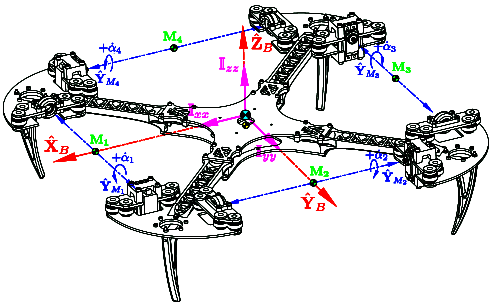
\includegraphics[width=0.9\textwidth]{figs/inertia-frame}
\caption{Inertial Center \& Mass Center}
\label{fig:inertia-frame}
\end{figure}
Each module's rotational center is spaced equally relative to $\vec{\mathbf{O}}_b$ with a parallel axis arm $\vec{L}_{arm}=\begin{bmatrix}
195.161 0 0
\end{bmatrix}^T~~[mm]$ (Fig:\ref{fig:inertia-frame}). The net inertial equation about $\vec{\mathbf{O}}_b$, dependent on a the actuator suite $\mathbb{U}$ positions, can be calculated as:
\begin{subequations}\label{eq:body-inertia}
\begin{equation}\label{eq:body-inertia.a}
\underset{u\in\mathbb{U}}{\mathbb{I}_b(u)}=\mathbb{I}_{body}+\sum_{i=1}^{4}\mathbb{M}_{i}~~[kg.m^2]
\end{equation}
\vspace{-10pt}
\begin{equation}\label{eq:body-inertia.b}
\mathbb{M}_i=\mathbb{I}_{i^{th}motor}+m_{module}\big(\vec{L} \cdot \vec{L} - \vec{L}\otimes\vec{L}\big)
\end{equation}
\end{subequations}
Although Eq:\ref{eq:body-inertia} does indeed produce the net body's inertia, the transformations to calculate $\mathbb{M}_i$ are compounded. Inertias are first translated to the center of rotation and then to the body frame's origin. Subsequent transformations are successively going to deteriorate the floating point precision of the resultant inertial tensor. Transforming inertial tensors about each sub-body's center of mass directly to the body frame origin is going to improve results. Similarly, it is more intuitive for the reader to consider each sub-body's contribution separately, despite having been derived as compound inertial systems previously. The relative movement pertinent to Eq:\ref{eq:inertia.inner} and Eq:\ref{eq:inertia.middle} are conceptually separated from that affecting Eq:\ref{eq:body-inertia}.  


It was found that each subsequent parallel axis translation further deteriorates the inertial value when compared to a true integral inertia. The net contributions used are translations of inertias from each respective center of mass to the origin $\vec{\mathbb{O}}\in\mathcal{F}^b$.
\begin{subequations}
\begin{equation}
\mathbb{M}_i=\mathbb{M}_{inner}+\mathbb{M}_{middle}
\end{equation}
For each inner ring, W.R.T its center of mass, different from Eq:\ref{eq:inertia.inner.a};
\begin{equation}
\underset{C.M}{\mathbb{I}_{inner}}=\begin{bmatrix}
585.11 & -0.34 & -2.44\\
-0.34 & 1960.93 & 0.81\\
-2.44 & 0.81 & 2139.84\\
\end{bmatrix}
\end{equation}
\begin{equation}
C.M_{inner}=\begin{bmatrix}
1.400 & -0.043 & -1.942
\end{bmatrix}^T~~[mm]
\end{equation}
\begin{equation}
\underset{||~\vec{\mathbf{O}}}{\mathbb{I}_{inner}}=\mathbb{R}_Z\mathbb{R}_y(\eta)\mathbb{R}_x(\lambda)\big(\mathbb{I}_{inner}\big)\mathbb{R}^{-1}_x(\lambda)\mathbb{R}^{-1}_y(\eta)\mathbb{R}^{-1}_Z
\end{equation}
\begin{equation}
\mathbb{M}_{inner}=\underset{\vec{\mathbf{O}}}{\mathbb{I}_{inner}}=\underset{||~\vec{\mathbf{O}}}{\mathbb{I}_{inner}}+ m \big((\Delta L \cdot \Delta L)\mathbb{I}_{3x3} - \Delta L \times \Delta L^{T} \big)
\end{equation}
\end{subequations}
Similarly for each middle ring:
\begin{subequations}
\begin{equation}
\underset{C.M}{\mathbb{I}_{middle}}=\begin{bmatrix}
2996.57 & 179.32 & 232.71\\
179.32 & 6524.84 & 13.87\\
232.71 & 13.87 & 9312.733\\
\end{bmatrix}
\end{equation}
\begin{equation}
C.M_{middle}=\begin{bmatrix}
47.00 & 3.74 & -3.63
\end{bmatrix}^T~~[mm]
\end{equation}
\begin{equation}
\mathbb{I}_{middle}=\underset{C.M}{\mathbb{I}_{middle}}+m_{middle}\big((\Delta_{C.M} \cdot \Delta_{C.M})\mathbb{I}_{3x3} - \Delta_{C.M} . \Delta_{C.M} ^T \big)
\end{equation}
\begin{equation}
\underset{||\vec{\mathbf{O}}}{\mathbb{I}_{middle}}=\mathbb{R}_Z\mathbb{R}_y(\eta)\big(\mathbb{I}_{middle}\big)\mathbb{R}^{-1}_y(\eta)\mathbb{R}^{-1}_Z
\end{equation}
\begin{equation}
\mathbb{M}_{i}=\underset{||\vec{\mathbf{O}}}{\mathbb{I}_{middle}}+m_{middle}\big((\Delta_{L}\cdot\Delta_{L})\mathbb{I}_{3x3}-\Delta_{L}.\Delta_{L}^T\big)
\end{equation}
\end{subequations}
The above equations begin to deviate from the true inertial value, the deviations stem from subsequent transformations.
\begin{subequations}
\begin{equation}
\mathbb{M}_i=\mathbb{R}(\sigma_i,~\eta_i)\big(\mathbb{I}_{middle}+\mathbb{R}_X(\lambda_i)(\mathbb{I}_{inner})\mathbb{R}_X^{-1}(\lambda_i)\big)\mathbb{R}^{-1}(\sigma_i,~\eta_i)+L_im_i^2
\end{equation}
\vspace{-10pt}
\begin{equation}
\sigma_i=\big[0^{\circ},~90^{\circ},~180^{\circ},~270^{\circ}\big]~\text{for}~i=[1:4]
\end{equation}
\end{subequations}
Unless otherwise stated, any inertia $\mathbb{I}_b$, irrespective of the arguments listed, refers to Eq:\ref{eq:body-inerta}.

\subsubsection*{Mass \& Center of Gravity}
Seeing as the servo and bearings in $\mathcal{F}^{M_i'}$ are unbalanced, the center of gravity isn't coincidental with the center of rotation. The offset position of the center of gravity is going to produce a gravitational torque arm about the motor modules axes.


%====================================================
\subsection{Actuator Transfer Functions}
\label{subsec:proto.design.transfer}
%====================================================

%====================================================
\subsection{Overall Aspects}
\label{subsec:proto.design.aspects}
%====================================================
\subsubsection{Vibration Damping}
%====================================================
\subsubsection{Landing Skids}
%====================================================
\subsubsection{Motors \& ESCs}
%====================================================

%====================================================
\section{System Layout}
\label{sec:proto.layout}
%====================================================
\subsection{Electrical Design}
\subsection{Component Characteristics}